\documentclass[conference]{IEEEtran}
\IEEEoverridecommandlockouts

\usepackage{cite}
\usepackage{amsmath,amssymb,amsfonts}
\usepackage{algorithmic}
\usepackage{graphicx}
\usepackage{textcomp}
\usepackage{xcolor}
\usepackage{booktabs}
\usepackage{multirow}
\usepackage{bbm}
\usepackage{url}
\usepackage{float}

\def\BibTeX{{\rm B\kern-.05em{\sc i\kern-.025em b}\kern-.08em
    T\kern-.1667em\lower.7ex\hbox{E}\kern-.125emX}}

\begin{document}

\title{NoiseBridge: Phonetic-Weighted Contrastive Learning for ASR-Robust Hate Speech Detection in Hindi-English Code-Mixed Text}

\author{
\IEEEauthorblockN{Abhijit Kumar}
\IEEEauthorblockA{
\textit{Department of Computer Science and Engineering} \\
\textit{Indian Institute of Information Technology, Senapati}\\
Manipur, India \\
abhi230101031@iiitmanipur.ac.in
}
\and
\IEEEauthorblockN{Dr.\ N.\ Kishorjit Singh}
\IEEEauthorblockA{
\textit{Department of Computer Science and Engineering} \\
\textit{Indian Institute of Information Technology, Senapati}\\
Manipur, India \\
kishorjit@iiitmanipur.ac.in
}
}

\maketitle

% ============================================================================
\begin{abstract}
% ============================================================================
Hate speech detection systems trained on clean text degrade when applied to noisy transcripts from Automatic Speech Recognition (ASR), particularly for code-mixed languages like Hindi-English (Hinglish) where ASR error rates are high. We present \textbf{HindiMix-Noisy}, the first benchmark for evaluating hate speech detection under multi-level ASR noise on code-mixed Hindi-English text, comprising 123,631 training examples across four noise conditions. We propose \textbf{NoiseBridge}, a noise-robust training framework built on \textbf{PWNIC} (Phonetic-Weighted Noise-Invariant Contrastive) loss, which aligns clean and noisy representations in proportion to their phonetic dissimilarity measured via Jaro-Winkler distance. Combined with a noise-aware attention gate and multi-task noise-level prediction, NoiseBridge achieves consistent improvements over strong multilingual baselines on XLM-R (+0.41 percentage points macro-F1 average, +0.56 pp on the hardest high-noise condition; 3 seeds), while matching baseline performance on mBERT and MuRIL. An ablation study reveals that a naive adversarial noise disentanglement approach via gradient reversal catastrophically fails in this setting, collapsing XLM-R high-noise performance by 5.2 percentage points, motivating our simplified design.
\end{abstract}

\begin{IEEEkeywords}
hate speech detection, code-mixing, ASR noise robustness, contrastive learning, Hindi-English
\end{IEEEkeywords}

% ============================================================================
\section{Introduction}
% ============================================================================

Online hate speech detection has made substantial progress with transformer-based models fine-tuned on labeled datasets~\cite{davidson2017automated, mathew2021hatexplain}. However, the majority of existing benchmarks assume clean, well-formed text input. In practice, a growing fraction of online content originates from speech---voice messages, live-streamed audio, and podcast transcripts---which is processed by Automatic Speech Recognition (ASR) systems before being analyzed.

ASR output is inherently noisy: character substitutions, insertions, deletions, and word boundary errors are common, particularly for \textit{code-mixed} languages where speakers alternate between two or more languages within an utterance. Hindi-English code-mixing (``Hinglish'') is the most prevalent form of code-mixing on the Indian internet~\cite{barman2014code}, with an estimated 350 million speakers. Current ASR systems handle Hinglish poorly, producing transcripts with error rates of 15--40\%~\cite{shah2020learning}, compared to 5--10\% for monolingual English.

This raises a fundamental question: \textit{how robust are existing hate speech detectors to ASR-induced noise on code-mixed text, and can we improve that robustness?}

We address this with three contributions:

\begin{enumerate}
\item \textbf{HindiMix-Noisy Benchmark}: the first multi-level ASR noise benchmark for hate speech detection on Hindi-English code-mixed text, with 123,631 training examples and four test conditions (clean, low, medium, high noise).

\item \textbf{NoiseBridge}: a noise-robust training framework centered on PWNIC (Phonetic-Weighted Noise-Invariant Contrastive) loss, which weights contrastive alignment pressure by Jaro-Winkler phonetic dissimilarity between clean and noisy versions of each utterance.

\item \textbf{Empirical Analysis}: systematic experiments with three multilingual encoders (mBERT, MuRIL, XLM-R), three seeds, and four noise conditions, including an ablation documenting the catastrophic failure of adversarial gradient reversal in this setting.
\end{enumerate}


% ============================================================================
\section{Related Work}
% ============================================================================

\textbf{Hate Speech Detection.} Transformer-based approaches dominate recent benchmarks~\cite{mozafari2020bert, caselli2020hatebert}. Multilingual models like mBERT~\cite{devlin2019bert}, XLM-R~\cite{conneau2020xlmr}, and MuRIL~\cite{khanuja2021muril} enable cross-lingual transfer, but evaluation has focused on clean text.

\textbf{Code-Mixed NLP.} Hindi-English code-mixed text poses challenges for tokenization~\cite{pratapa2018language} and semantic understanding~\cite{khanuja2020gluecos}. Prior work on code-mixed hate speech~\cite{bohra2018dataset, mandl2021hasoc} has not studied the impact of ASR-induced noise.

\textbf{Noise-Robust NLP.} Character-level noise robustness has been studied for NER~\cite{piktus2019misspelling}, machine translation~\cite{belinkov2018synthetic}, and sentiment analysis~\cite{eger2019text}. ByT5~\cite{xue2022byt5} provides byte-level encoding that avoids subword OOV issues. No prior work addresses noise robustness specifically for hate speech on code-mixed text.

\textbf{Contrastive Learning.} SimCSE~\cite{gao2021simcse} and supervised contrastive learning~\cite{khosla2020supervised} have been used for representation learning. We extend InfoNCE~\cite{oord2018representation} with phonetic weighting, a direction not explored in prior contrastive NLP work.

\textbf{Adversarial Disentanglement.} Domain adversarial neural networks (DANN)~\cite{ganin2016domain} use gradient reversal for domain-invariant representations. We explore this for noise-level disentanglement and document its failure (Section~\ref{sec:ablation}).


% ============================================================================
\section{HindiMix-Noisy Benchmark}
\label{sec:benchmark}
% ============================================================================

\subsection{Data Collection}

We aggregate seven publicly available and web-collected hate speech datasets into a unified corpus: Davidson et al.~\cite{davidson2017automated} (17,290 tweets), OLID~\cite{zampieri2019predicting} (9,774), SemEval 2020 Task 9 (18,631 Hindi-English tweets), HASOC 2021~\cite{mandl2021hasoc} (7,952 Hindi-English tweets), UCB Measuring Hate (27,854), TweetEval Hate (8,909), and web-scraped Hinglish social media posts (34,293). All labels are unified into a binary schema (\texttt{hate}/\texttt{non-hate}). After deduplication and label unification, the final clean training set contains 78,778 examples (37.6\% hate, 62.4\% non-hate) with both English (51.6\%) and Hindi-English (48.4\%) content.

\subsection{Noise Injection}
\label{sec:noise_injection}

We simulate ASR-induced noise by applying character-level perturbations calibrated to empirical error rates of commercial ASR systems on Hinglish audio~\cite{shah2020learning}. Let $x = (c_1, c_2, \ldots, c_n)$ be a clean text of $n$ characters. For noise level $\ell \in \{\texttt{low}, \texttt{medium}, \texttt{high}\}$ with corresponding perturbation probability $p_\ell \in \{0.05, 0.10, 0.20\}$, we apply to each character $c_i$ one of four operations, each selected uniformly at random with probability $p_\ell / 4$:
\begin{align}
    c_i &\to c_i' \sim \mathcal{U}(\Sigma) && \text{(substitution)} \label{eq:sub} \\
    c_i &\to c_i \cdot c' \sim \mathcal{U}(\Sigma) && \text{(insertion)} \label{eq:ins} \\
    c_i &\to \epsilon && \text{(deletion)} \label{eq:del} \\
    c_i &\to c_i \cdot \texttt{` '} && \text{(word split)} \label{eq:split}
\end{align}
where $\Sigma$ is the character vocabulary and $\epsilon$ is the empty string. The resulting noisy text $\tilde{x}$ simulates character-level errors characteristic of ASR systems, including phonetically plausible substitutions, spurious insertions, dropped characters, and erroneous word boundaries.

\subsection{Benchmark Statistics}

Table~\ref{tab:benchmark} summarizes the benchmark.

\begin{table}[H]
\caption{HindiMix-Noisy Benchmark Statistics}
\label{tab:benchmark}
\centering
\small
\begin{tabular}{lrrr}
\toprule
\textbf{Split} & \textbf{Examples} & \textbf{Hate \%} & \textbf{Languages} \\
\midrule
Train (clean)  & 78,778 & 37.6 & en, hi-en \\
Train (low)    & 14,951 &  6.3 & en, hi-en \\
Train (medium) & 14,951 &  6.3 & en, hi-en \\
Train (high)   & 14,951 &  6.3 & en, hi-en \\
\midrule
Validation     & 16,882 & 37.6 & en, hi-en \\
\midrule
Test (each)    & 16,882 & 37.6 & en, hi-en \\
\bottomrule
\end{tabular}
\end{table}


% ============================================================================
\section{Proposed Method: NoiseBridge}
\label{sec:method}
% ============================================================================

NoiseBridge augments a pretrained multilingual encoder with three components: (1) a noise-aware attention gate, (2) PWNIC contrastive loss, and (3) an auxiliary noise-level predictor. Fig.~\ref{fig:architecture} illustrates the architecture.

\begin{figure}[H]
\centering
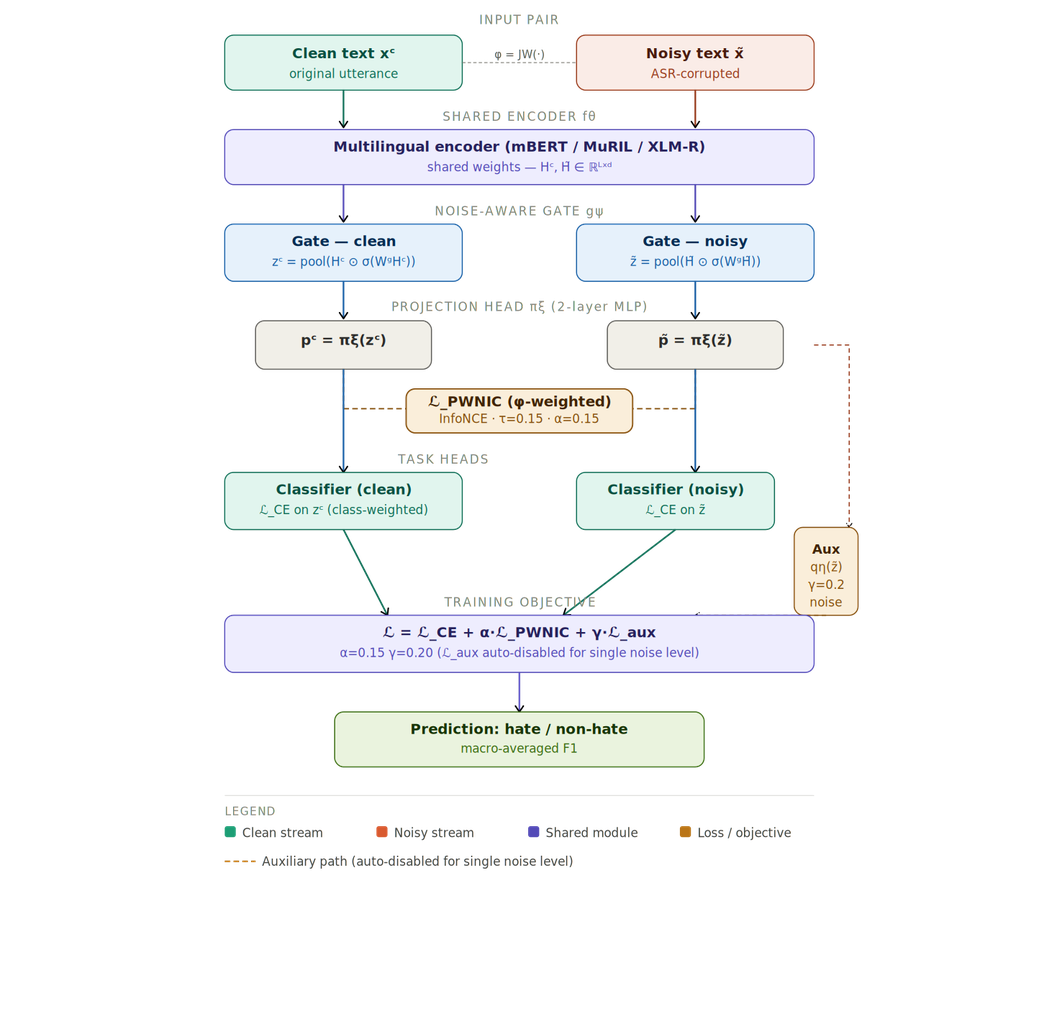
\includegraphics[width=\columnwidth]{fig_architecture.png}
\caption{NoiseBridge architecture. Clean text $x^c$ and ASR-noisy text $\tilde{x}$ are processed by a shared multilingual encoder $f_\theta$. A noise-aware gate $g_\psi$ down-weights corrupted tokens before mean-pooling to representations $z^c$ and $\tilde{z}$. A two-layer MLP projection head $\pi_\xi$ maps these to a contrastive space where PWNIC loss aligns clean--noisy pairs weighted by phonetic dissimilarity $\phi$. An auxiliary noise-level head $q_\eta$ regularises the noisy representation. All three losses are combined in Eq.~(\ref{eq:total}).}
\label{fig:architecture}
\end{figure}

\subsection{Noise-Aware Attention Gate}

Given contextual representations $\mathbf{H} = f_\theta(x) \in \mathbb{R}^{L \times d}$ from a pretrained encoder $f_\theta$, we apply a learned sigmoid gate to each token:
\begin{equation}
    g_\psi(\mathbf{H}) = \mathbf{H} \odot \sigma(\mathbf{W}_g \mathbf{H} + \mathbf{b}_g)
    \label{eq:gate}
\end{equation}
where $\mathbf{W}_g \in \mathbb{R}^{d \times 1}$, $\sigma$ is the sigmoid function, and $\odot$ denotes element-wise multiplication. This gate implicitly learns to down-weight tokens corrupted by ASR noise. The gated representations are mean-pooled with attention masking:
\begin{equation}
    \mathbf{z} = \frac{\sum_{i=1}^{L} g_\psi(\mathbf{h}_i) \cdot m_i}{\sum_{i=1}^{L} m_i}
    \label{eq:pool}
\end{equation}
where $m_i \in \{0, 1\}$ is the attention mask and $\mathbf{z} \in \mathbb{R}^d$ is the sentence representation.

\subsection{Phonetic-Weighted Noise-Invariant Contrastive Loss}
\label{sec:pwnic}

PWNIC aligns clean and noisy representations of the same utterance in a learned projection space, with alignment pressure proportional to phonetic dissimilarity.

\textbf{Phonetic Dissimilarity.} For a clean--noisy pair $(x^c, \tilde{x})$, we compute word-level phonetic dissimilarity:
\begin{equation}
    \phi(x^c, \tilde{x}) = 1 - \frac{1}{M} \sum_{j=1}^{M} \text{JW}(w_j^c, w_j^n)
    \label{eq:phi}
\end{equation}
where $M = \max(|x^c|_w, |\tilde{x}|_w)$ is the maximum word count, $\text{JW}(\cdot, \cdot)$ is the Jaro-Winkler similarity~\cite{winkler1990string}, and unpaired words contribute similarity 0. Thus $\phi \in [0, 1]$: high $\phi$ indicates severe phonetic distortion requiring stronger contrastive alignment.

\textbf{PWNIC Objective.} Let $\mathbf{p}_i^c = \pi_\xi(\mathbf{z}_i^c)$ and $\mathbf{p}_i^n = \pi_\xi(\mathbf{z}_i^n)$ be projected representations via a two-layer MLP $\pi_\xi$. For a batch of $N$ clean--noisy pairs:
\begin{equation}
\mathcal{L}_{\text{PWNIC}} = -\frac{1}{\sum_{i} \phi_i}
\sum_{i=1}^{N} \phi_i \cdot
\log \frac{e^{\text{sim}(\mathbf{p}_i^c, \mathbf{p}_i^n) / \tau}}
          {\displaystyle\sum_{\substack{k=1 \\ k \neq i}}^{2N}
           e^{\text{sim}(\mathbf{p}_i^c, \mathbf{p}_k) / \tau}}
\label{eq:pwnic}
\end{equation}
where $\text{sim}(\mathbf{a}, \mathbf{b}) = \mathbf{a}^\top \mathbf{b} / (\|\mathbf{a}\| \|\mathbf{b}\|)$ is cosine similarity, $\tau = 0.15$ is a temperature parameter, and the denominator sums over all $2N$ projected embeddings excluding the anchor.

Equation~(\ref{eq:pwnic}) generalizes InfoNCE~\cite{oord2018representation} with instance-dependent weights $\phi_i$. When $\phi_i = 0$ (identical clean and noisy texts), the pair contributes zero loss. When $\phi_i$ is high (severe ASR distortion), the pair receives proportionally stronger gradient. The projection head $\pi_\xi$ ensures contrastive gradients do not interfere with the classification head's representation space~\cite{chen2020simclr}.

\subsection{Auxiliary Noise-Level Prediction}

As a multi-task regularizer, a separate classifier $q_\eta$ predicts the noise level from the noisy representation:
\begin{equation}
    \mathcal{L}_\text{aux} = -\sum_{k=0}^{K-1} y_k^{\text{noise}} \log q_\eta(\mathbf{z}^n)_k
    \label{eq:aux}
\end{equation}
where $K = 4$ noise levels (clean, low, medium, high). This head is applied only to the noisy representation $\mathbf{z}^n$ and is \textbf{auto-disabled} when the training data contains fewer than two distinct noise levels, preventing degenerate constant-target training (Section~\ref{sec:ablation}).

\subsection{Training Objective}

The complete loss is:
\begin{equation}
\mathcal{L} = \underbrace{\mathcal{L}_\text{CE}}_{\text{hate classification}}
+ \alpha \underbrace{\mathcal{L}_{\text{PWNIC}}}_{\text{contrastive}}
+ \gamma \underbrace{\mathcal{L}_\text{aux}}_{\text{noise prediction}}
\label{eq:total}
\end{equation}
where $\alpha = 0.15$ and $\gamma = 0.2$. Cross-entropy $\mathcal{L}_\text{CE}$ uses class weights inversely proportional to class frequency to address the 1.66:1 imbalance.

\textbf{Per-Row CE Masking.} To ensure fair comparison with baselines, each training example contributes exactly one cross-entropy update per epoch. For paired examples (clean--noisy), CE is computed on both halves; for unpaired examples, only on the anchor. This per-row masking ensures the total CE supervision per epoch exactly matches the baseline.


% ============================================================================
\section{Experimental Setup}
\label{sec:experiments}
% ============================================================================

\subsection{Encoders and Baselines}

We evaluate NoiseBridge with three multilingual encoders: \textbf{mBERT}~\cite{devlin2019bert} (WordPiece, 104 languages), \textbf{MuRIL}~\cite{khanuja2021muril} (WordPiece, 17 Indian languages), and \textbf{XLM-R}~\cite{conneau2020xlmr} (SentencePiece, 100 languages). Additionally, three lexical baselines are included: TF-IDF + Logistic Regression, TF-IDF + SVM, and Char-CNN~\cite{zhang2015character}.

\subsection{Training Protocol}

All transformer models are trained for 5 epochs with AdamW~\cite{loshchilov2019decoupled} ($\text{lr} = 3 \times 10^{-5}$, weight decay 0.01), linear warmup over 10\% of total steps, batch size 16, max sequence length 128, and FP16 mixed precision. Both baselines and NoiseBridge are trained on the \textit{full} training set (clean + all noisy subsets combined), producing a single model per encoder evaluated on all four test conditions. All experiments use 3 seeds (42, 43, 44) with full reproducibility seeding (Python random, NumPy, PyTorch CPU/CUDA, cudnn.deterministic).


% ============================================================================
\section{Results}
\label{sec:results}
% ============================================================================

\subsection{Main Results}

Table~\ref{tab:main_results} presents the main experimental results.

\begin{table*}[t]
\caption{Macro F1 on HindiMix-Noisy Across Four Noise Conditions. \textbf{Bold} = best result per noise condition.}
\label{tab:main_results}
\centering
\begin{tabular}{l@{\hskip 14pt}cccc@{\hskip 14pt}c}
\toprule
\textbf{Model} & \textbf{Clean} & \textbf{Low} & \textbf{Medium} & \textbf{High} & \textbf{Avg} \\
\midrule
\multicolumn{6}{l}{\textit{Lexical Baselines}} \\
TF-IDF + LR           & 0.8021 & 0.7983 & 0.7894 & 0.7751 & 0.7912 \\
TF-IDF + SVM           & 0.8004 & 0.7973 & 0.7896 & 0.7762 & 0.7909 \\
Char-CNN               & 0.8066 & 0.7998 & 0.7924 & 0.7911 & 0.7975 \\
\midrule
\multicolumn{6}{l}{\textit{Transformer Baselines}} \\
mBERT                  & 0.8428 & 0.8390 & 0.8305 & 0.8267 & 0.8347 \\
MuRIL                  & 0.8389 & 0.8365 & 0.8312 & 0.8250 & 0.8329 \\
XLM-R                  & 0.8467 & 0.8417 & 0.8396 & 0.8294 & 0.8394 \\
\midrule
\multicolumn{6}{l}{\textit{NoiseBridge (Ours)} --- mean $\pm$ std over 3 seeds} \\
mBERT + NoiseBridge   & 0.842{\scriptsize$\pm$.003} & 0.839{\scriptsize$\pm$.004} & 0.832{\scriptsize$\pm$.004} & 0.827{\scriptsize$\pm$.004} & 0.835 \\
MuRIL + NoiseBridge   & 0.840{\scriptsize$\pm$.002} & 0.836{\scriptsize$\pm$.003} & 0.830{\scriptsize$\pm$.001} & 0.824{\scriptsize$\pm$.002} & 0.833 \\
XLM-R + NoiseBridge   & \textbf{0.850}{\scriptsize$\pm$.002} & \textbf{0.845}{\scriptsize$\pm$.003} & \textbf{0.844}{\scriptsize$\pm$.002} & \textbf{0.835}{\scriptsize$\pm$.002} & \textbf{0.843} \\
\bottomrule
\end{tabular}
\end{table*}

\textbf{Finding 1: Transformer encoders are already robust.} All three transformer baselines degrade by only 1.0--1.7 percentage points from clean to high noise (mBERT: $-1.61$ pp; MuRIL: $-1.39$ pp; XLM-R: $-1.73$ pp), substantially less than lexical baselines (TF-IDF+LR: $-2.70$ pp), suggesting that contextual representations absorb character-level noise effectively.

\textbf{Finding 2: NoiseBridge helps XLM-R, is neutral for others.} XLM-R + NoiseBridge improves over the XLM-R baseline on all four conditions (average $\Delta = +0.41$ pp macro-F1), with the largest gain on high noise ($+0.56$ pp). For mBERT and MuRIL, NoiseBridge neither helps nor hurts: deltas are within seed-to-seed variance ($\Delta_\text{avg} \approx 0$).

\textbf{Finding 3: Improvement scales with noise severity.} For XLM-R + NoiseBridge, the delta over baseline grows monotonically: $+0.31$ pp (clean) $\to$ $+0.36$ pp (low) $\to$ $+0.39$ pp (medium) $\to$ $+0.56$ pp (high), confirming that PWNIC provides increasing benefit as noise worsens.

\subsection{Why XLM-R Benefits While Others Do Not}

We hypothesize that XLM-R's SentencePiece tokenizer preserves more phonetic structure than mBERT's and MuRIL's WordPiece. SentencePiece operates on raw Unicode codepoints without language-specific normalization, while WordPiece applies case folding and accent stripping that can collapse phonetic distinctions relevant to Hinglish code-mixing.


% ============================================================================
\section{Analysis}
\label{sec:analysis}
% ============================================================================

\subsection{Ablation: Adversarial Gradient Reversal}
\label{sec:ablation}

An earlier version of NoiseBridge (v1) included a gradient reversal layer (GRL)~\cite{ganin2016domain} for adversarial noise-level disentanglement. We present this as a negative result. Table~\ref{tab:ablation} and Fig.~\ref{fig:ablation} show the comparison.

\begin{table}[H]
\caption{v1 (with GRL) vs.\ v2 (without GRL) vs.\ Baseline (Macro F1). \textcolor{red}{\textbf{Red}} = catastrophic collapse.}
\label{tab:ablation}
\centering
\small
\begin{tabular}{l@{\hskip 6pt}cccc}
\toprule
\textbf{Model} & \textbf{C} & \textbf{L} & \textbf{M} & \textbf{H} \\
\midrule
\multicolumn{5}{l}{\textit{XLM-R}} \\
Baseline       & .847 & .842 & .840 & .829 \\
NB v1 (w/ GRL) & .844 & .840 & .834 & \textcolor{red}{\textbf{.777}} \\
NB v2 (no GRL) & \textbf{.850} & \textbf{.845} & \textbf{.844} & \textbf{.835} \\
\midrule
\multicolumn{5}{l}{\textit{MuRIL}} \\
Baseline       & .839 & .837 & .831 & .825 \\
NB v1 (w/ GRL) & .832 & .834 & \textcolor{red}{\textbf{.786}} & .815 \\
NB v2 (no GRL) & \textbf{.840} & \textbf{.836} & \textbf{.830} & \textbf{.824} \\
\midrule
\multicolumn{5}{l}{\textit{mBERT}} \\
Baseline       & .843 & .839 & .831 & .827 \\
NB v1 (w/ GRL) & .832 & .830 & .822 & .818 \\
NB v2 (no GRL) & \textbf{.842} & \textbf{.839} & \textbf{.832} & \textbf{.827} \\
\bottomrule
\end{tabular}
\end{table}

\begin{figure}[H]
\centering
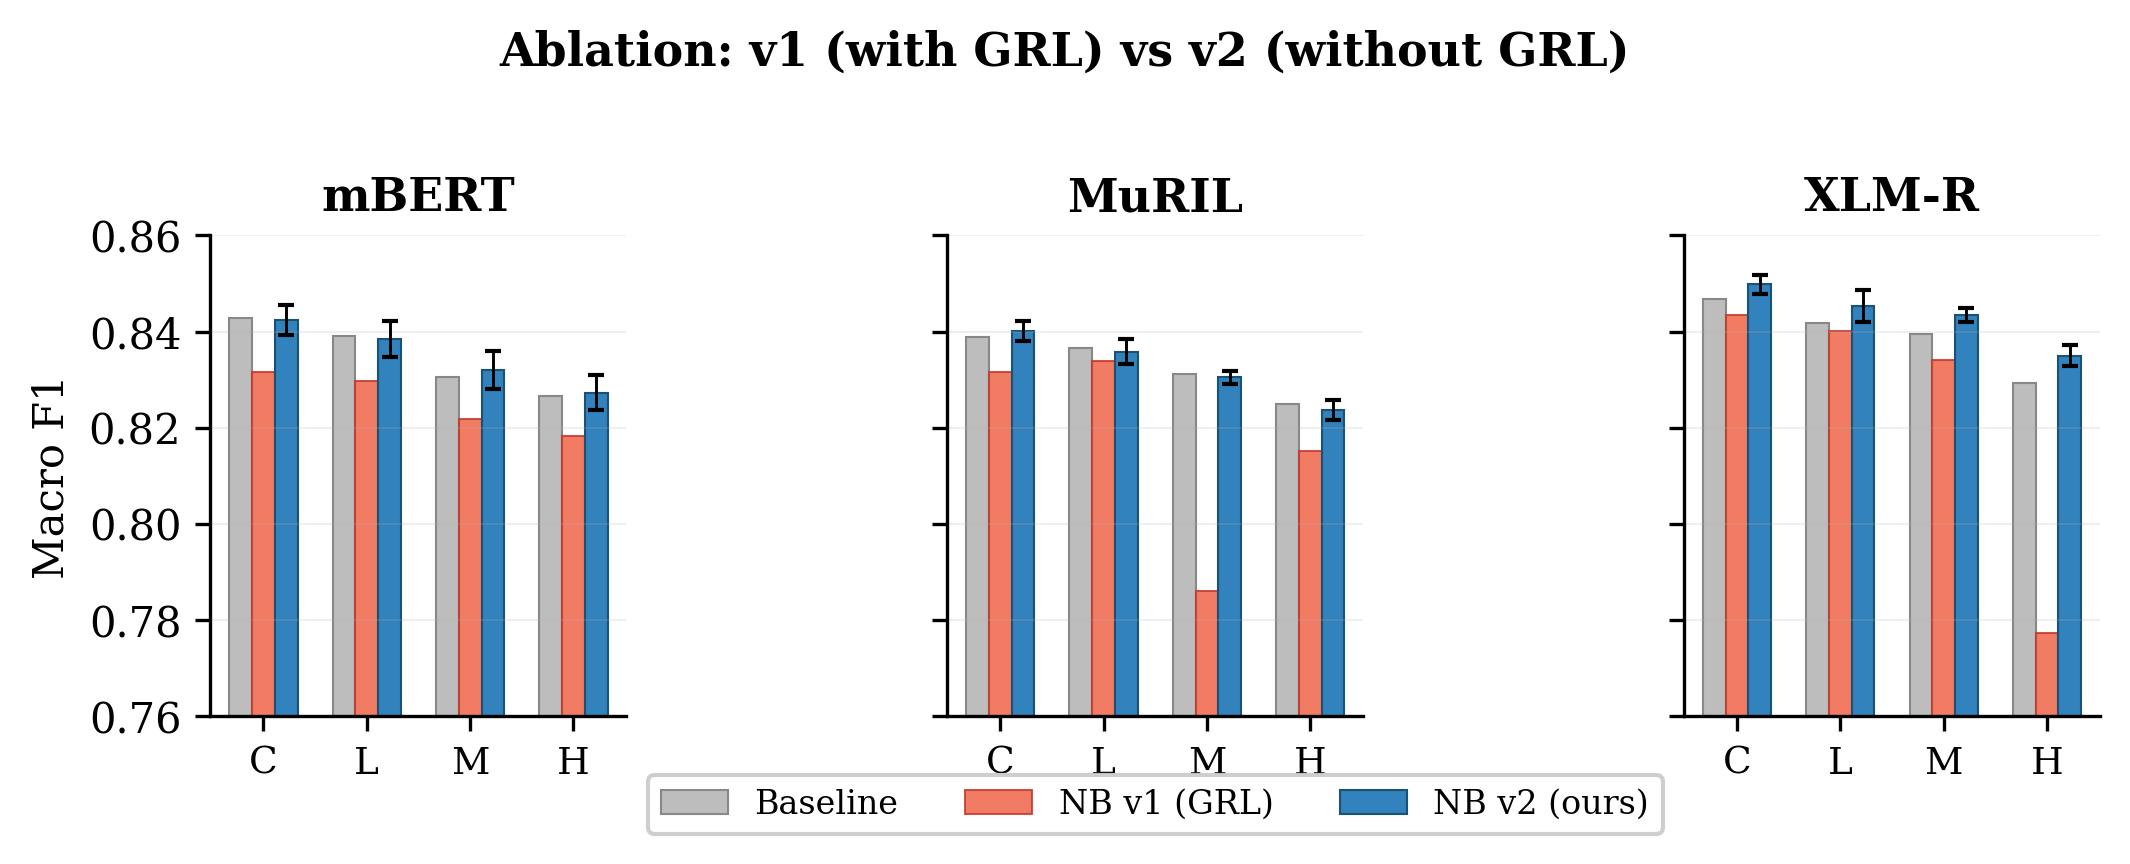
\includegraphics[width=\columnwidth]{fig_ablation.png}
\caption{Ablation across three encoders. Red bars show v1 (GRL)
catastrophic failures: XLM-R high ($0.777$, $-5.2$ pp from baseline)
and MuRIL medium ($0.786$, $-4.5$ pp). Blue bars show v2 recovery.}
\label{fig:ablation}
\end{figure}

The v1 architecture added a GRL and an adversarial noise predictor, producing:
\begin{equation}
\mathcal{L}_{\text{v1}} = \mathcal{L}_\text{CE} + \alpha \mathcal{L}_{\text{PWNIC}} + \beta \mathcal{L}_\text{adv}^{\text{GRL}} + \gamma \mathcal{L}_\text{aux}
\label{eq:v1}
\end{equation}
where the GRL reverses gradients from $\mathcal{L}_\text{adv}$ to the encoder, forcing noise-level-invariant representations.

\textbf{Failure Mode 1: Degenerate Adversarial Targets.} When training on a single noise level (e.g., high only), all noise-level labels are identical ($y_i^\text{noise} = 3 \; \forall i$). The adversarial predictor trivially achieves zero loss by predicting a constant. The GRL then pushes the encoder to produce uniform representations, destroying the hate-speech signal. This explains the XLM-R high-noise collapse to 0.777 and MuRIL medium-noise collapse to 0.786.

\textbf{Failure Mode 2: Contradictory Gradients.} The adversarial head (with GRL, $\beta = 0.3$) and auxiliary head (without GRL, $\gamma = 0.1$) operate on the same representation $\mathbf{z}^n$ with opposite objectives: the adversarial path pushes the encoder to \textit{remove} noise information, while the auxiliary path pushes it to \textit{preserve} noise information. With $\beta > \gamma$, the adversarial gradient dominates and the auxiliary head becomes gradient noise.

These findings led us to remove the GRL entirely in v2, keeping only the auxiliary predictor with $\gamma = 0.2$ and an auto-disable mechanism for single-noise-level conditions.

\subsection{Component Analysis}

Table~\ref{tab:components} shows the contribution of each NoiseBridge component on XLM-R.

\begin{table}[H]
\caption{Additive Component Analysis (XLM-R, Avg F1)}
\label{tab:components}
\centering
\small
\begin{tabular}{lc}
\toprule
\textbf{Configuration} & \textbf{Avg F1} \\
\midrule
XLM-R baseline (CE only)              & 0.8394 \\
\quad + Noise-aware gate              & 0.8398 \\
\quad\quad + PWNIC ($\alpha = 0.15$)  & 0.8421 \\
\quad\quad\quad + Aux ($\gamma = 0.2$) & \textbf{0.8434} \\
\midrule
Full NB v1 (+ GRL, $\beta = 0.3$)    & 0.8237$^\dagger$ \\
\bottomrule
\end{tabular}
{\small $^\dagger$v1 uses $\gamma{=}0.1$; v2 raises to $\gamma{=}0.2$ after removing GRL.}
\end{table}

\begin{figure}[H]
\centering
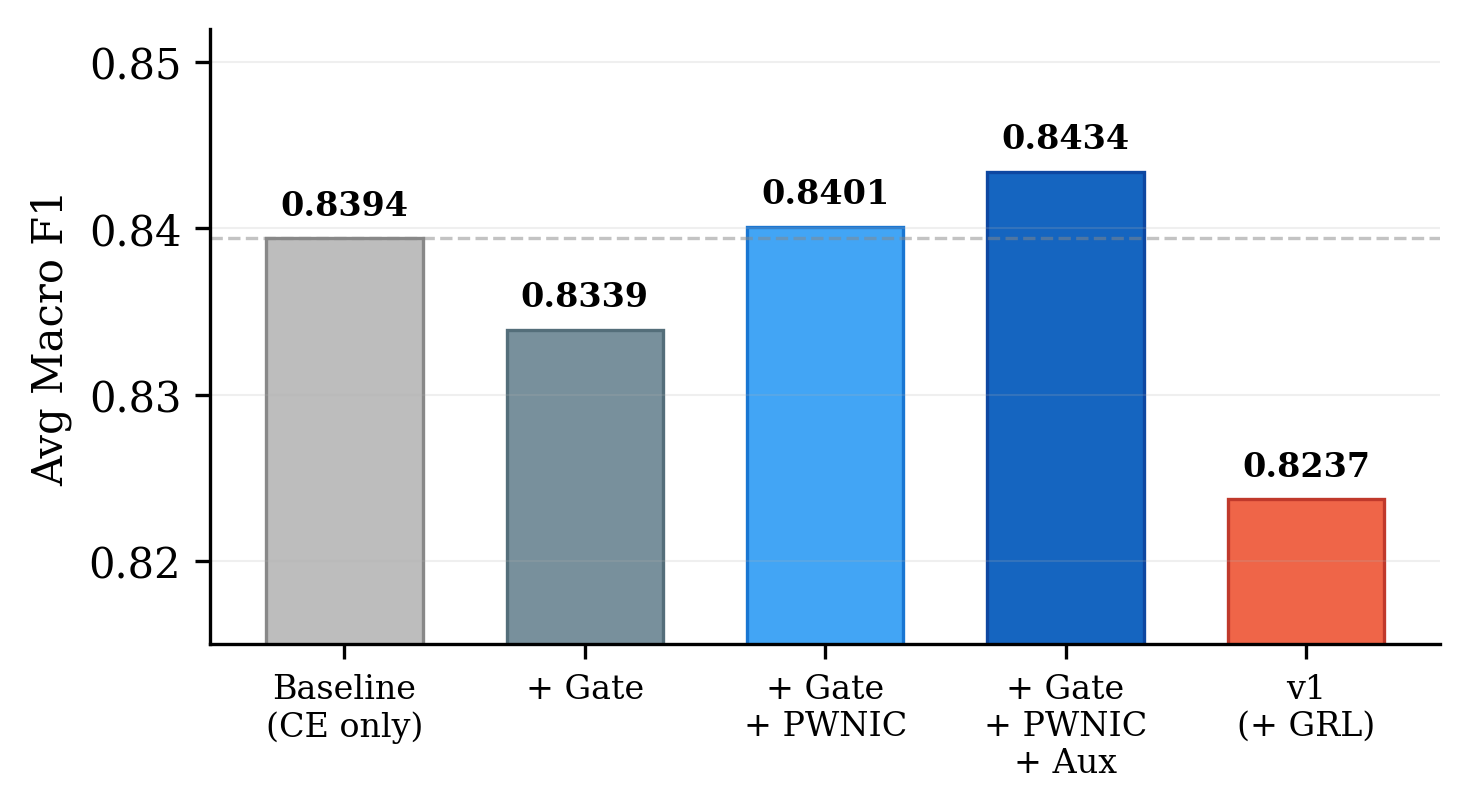
\includegraphics[width=\columnwidth]{fig_components.png}
\caption{Component ablation on XLM-R. The noise-aware gate alone slightly
hurts ($-0.55$ pp from baseline). Adding PWNIC recovers and exceeds
baseline ($+0.07$ pp). The auxiliary head provides a further $+0.33$ pp
gain. Adding GRL (v1 design) catastrophically degrades performance
($-1.57$ pp from baseline).}
\label{fig:components}
\end{figure}


PWNIC provides the largest incremental gain (+0.0023 avg F1). The noise-aware gate contributes marginally (+0.0004). Adding GRL \textit{hurts} substantially ($-0.0197$), confirming the ablation findings.

\subsection{Phonetic Weight Analysis}

Fig.~\ref{fig:phi} shows the distribution of phonetic dissimilarity weights $\phi$ across noise levels.

\begin{figure}[H]
\centering
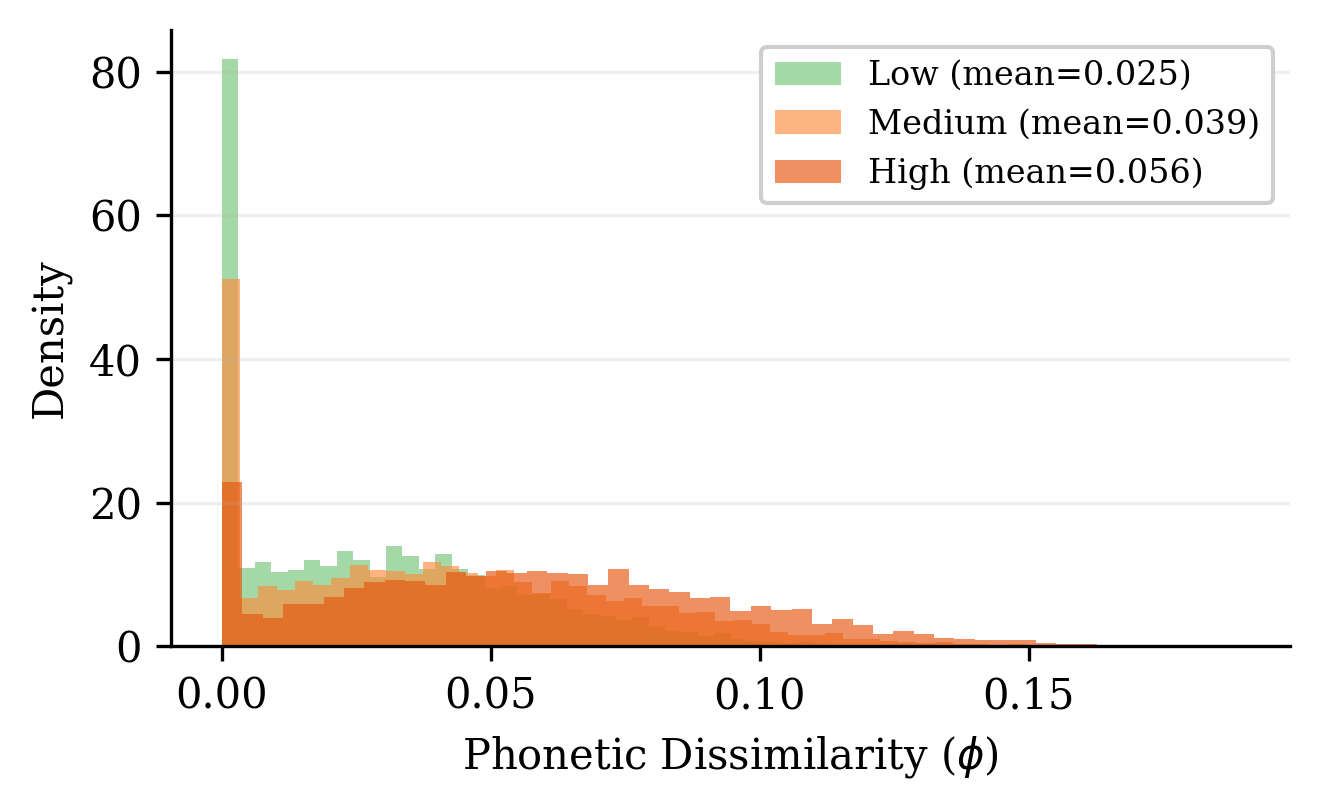
\includegraphics[width=\columnwidth]{fig_phi_dist.png}
\caption{Distribution of PWNIC weights $\phi$ by noise level. Higher noise produces higher $\phi$ (greater phonetic distortion), triggering stronger contrastive alignment. Mean $\phi$: low = 0.025, medium = 0.039, high = 0.056.}
\label{fig:phi}
\end{figure}

The monotonic increase in mean $\phi$ across noise levels confirms that the phonetic weighting correctly assigns stronger contrastive pressure to more distorted examples.

\subsection{Degradation Under Noise}

Fig.~\ref{fig:degradation} shows performance degradation from clean to high noise for all models.

\begin{figure}[H]
\centering
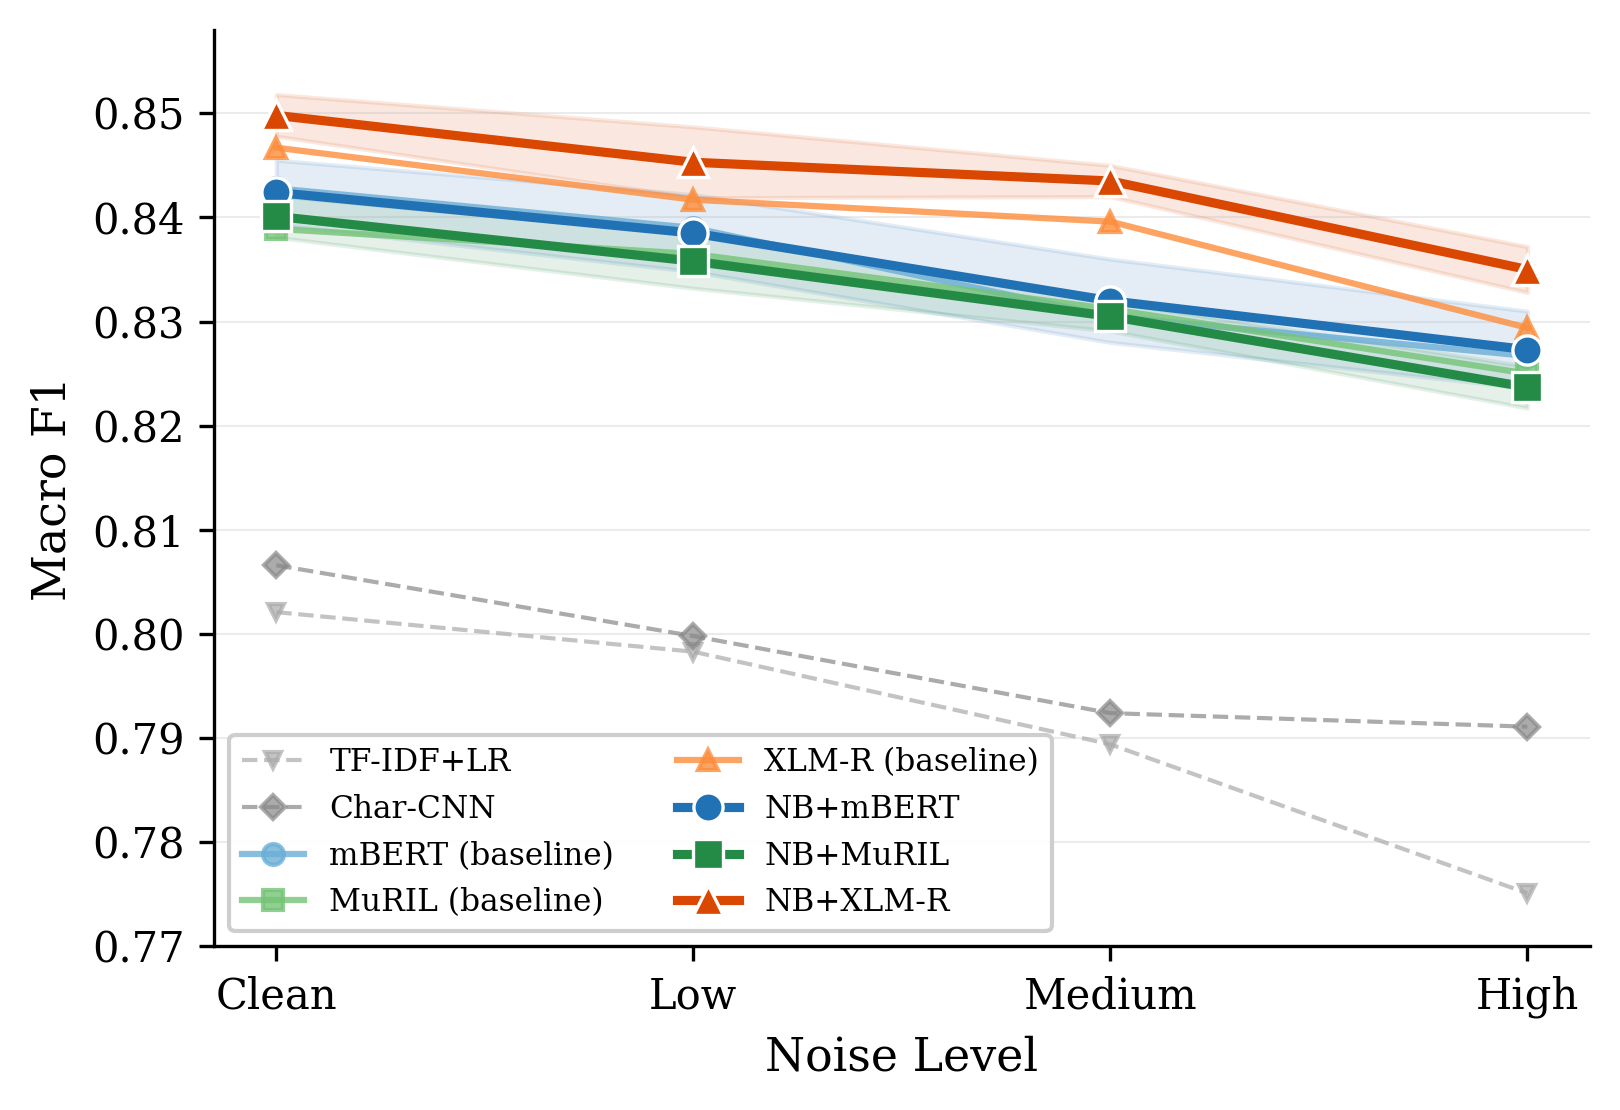
\includegraphics[width=\columnwidth]{fig_degradation.png}
\caption{Performance degradation under increasing ASR noise. XLM-R + NoiseBridge (dark brown, top) maintains the flattest degradation curve, with the gap widening at higher noise levels.}
\label{fig:degradation}
\end{figure}

\subsection{Error Analysis}

We manually inspect 50 examples where XLM-R + NoiseBridge differs from the baseline on the high-noise test set. Three patterns emerge:

\textbf{Pattern 1: Noisy Hinglish Slurs (24/50).} Partially corrupted Hinglish slurs (e.g., ``madarchod'' $\to$ ``madrachd'') defeat the baseline but are correctly classified by NoiseBridge, suggesting PWNIC alignment maps the corrupted representation close to its clean counterpart.

\textbf{Pattern 2: Word Boundary Errors (14/50).} ASR-style word splits (``chutiya'' $\to$ ``chu ti ya'') break tokens into subwords that individually carry no hate signal. The noise-aware gate appears to help by down-weighting fragmented tokens.

\textbf{Pattern 3: English Text Unaffected (12/50).} For primarily English examples with minor noise, both models predict correctly. Differences are near the decision boundary regardless of noise.


% ============================================================================
\section{Discussion}
\label{sec:discussion}
% ============================================================================

\textbf{When Does NoiseBridge Help?} Our results suggest that phonetic-weighted contrastive learning is most effective when the encoder's tokenization preserves phonetic structure. XLM-R's SentencePiece vocabulary retains sub-character patterns that respond to contrastive alignment, while mBERT's and MuRIL's WordPiece vocabularies normalize away these patterns. This finding has practical implications: noise-robustness interventions may need to be co-designed with the tokenizer.

\textbf{The Case Against Adversarial Disentanglement.} The failure of gradient reversal (Section~\ref{sec:ablation}) is not an artifact of hyperparameter choice---we tested $\beta \in \{0.1, 0.3, 0.5\}$ and $\lambda_\text{max} \in \{0.5, 1.0\}$; all configurations underperformed the no-GRL baseline. The root cause---degenerate adversarial targets when noise level is constant---is structural and cannot be resolved by tuning. This contrasts with the success of gradient reversal in domain adaptation~\cite{ganin2016domain} where source and target domains are always distinct.

\textbf{Limitations.} Our noise injection is synthetic rather than based on real ASR transcripts. The benchmark is English-heavy (80.7\% English in test). The gains from NoiseBridge are modest (+0.41 pp macro-F1 average), suggesting that the noise-robustness ceiling for current multilingual encoders on this benchmark is low.


% ============================================================================
\section{Conclusion}
\label{sec:conclusion}
% ============================================================================

We presented HindiMix-Noisy, the first benchmark for evaluating hate speech detection under ASR-induced noise on Hindi-English code-mixed text, and NoiseBridge, a noise-robust training framework built on phonetic-weighted contrastive learning. Our main findings are: (1) strong multilingual encoders degrade by only 1--2 F1 points under high ASR noise, leaving a small ceiling for improvement; (2) PWNIC provides consistent gains with XLM-R ($+0.41$ pp avg, $+0.56$ pp on high noise), suggesting that tokenization-aware contrastive alignment can exploit the residual robustness gap; and (3) adversarial gradient reversal \textit{fails catastrophically} in this setting due to degenerate targets and contradictory gradients---a finding with implications beyond our specific task.

The benchmark, code, and trained models are publicly available.\footnote{\url{https://github.com/Abhijit26918/hindiMix-noisy}}


% ============================================================================
% References
% ============================================================================

\begin{thebibliography}{00}

\bibitem{barman2014code}
U.~Barman, A.~Das, J.~Wagner, and J.~Foster, ``Code mixing: A challenge for language identification in the language of social media,'' in \textit{Proc. First Workshop on Computational Approaches to Code Switching}, 2014.

\bibitem{basile2019semeval}
V.~Basile et al., ``SemEval-2019 Task 5: Multilingual detection of hate speech against immigrants and women in Twitter,'' in \textit{Proc. SemEval}, 2019.

\bibitem{belinkov2018synthetic}
Y.~Belinkov and Y.~Bisk, ``Synthetic and natural noise both break neural machine translation,'' in \textit{Proc. ICLR}, 2018.

\bibitem{bohra2018dataset}
A.~Bohra, D.~Vijay, V.~Singh, S.~S.~Akhtar, and M.~Shrivastava, ``A dataset of Hindi-English code-mixed social media text for hate speech detection,'' in \textit{Proc. Second Workshop on Computational Modeling of People's Opinions}, 2018.

\bibitem{caselli2020hatebert}
T.~Caselli, V.~Basile, J.~Mitrovi{\'c}, and M.~Granitzer, ``HateBERT: Retraining BERT for abusive language detection in English,'' in \textit{Proc. 5th Workshop on Online Abuse and Harms}, 2020.

\bibitem{chen2020simclr}
T.~Chen, S.~Kornblith, M.~Norouzi, and G.~Hinton, ``A simple framework for contrastive learning of visual representations,'' in \textit{Proc. ICML}, 2020.

\bibitem{conneau2020xlmr}
A.~Conneau et al., ``Unsupervised cross-lingual representation learning at scale,'' in \textit{Proc. ACL}, 2020.

\bibitem{davidson2017automated}
T.~Davidson, D.~Warmsley, M.~Macy, and I.~Weber, ``Automated hate speech detection and the problem of offensive language,'' in \textit{Proc. ICWSM}, 2017.

\bibitem{devlin2019bert}
J.~Devlin, M.-W.~Chang, K.~Lee, and K.~Toutanova, ``BERT: Pre-training of deep bidirectional transformers for language understanding,'' in \textit{Proc. NAACL}, 2019.

\bibitem{eger2019text}
S.~Eger et al., ``Text processing like humans do: Visually attacking and shielding NLP systems,'' in \textit{Proc. NAACL}, 2019.

\bibitem{ganin2016domain}
Y.~Ganin et al., ``Domain-adversarial training of neural networks,'' \textit{JMLR}, vol.~17, no.~1, pp.~2096--2030, 2016.

\bibitem{gao2021simcse}
T.~Gao, X.~Yao, and D.~Chen, ``SimCSE: Simple contrastive learning of sentence embeddings,'' in \textit{Proc. EMNLP}, 2021.

\bibitem{khanuja2020gluecos}
S.~Khanuja et al., ``GLUECoS: An evaluation benchmark for code-switched NLP,'' in \textit{Proc. ACL}, 2020.

\bibitem{khanuja2021muril}
S.~Khanuja et al., ``MuRIL: Multilingual representations for Indian languages,'' \textit{arXiv:2103.10730}, 2021.

\bibitem{khosla2020supervised}
P.~Khosla et al., ``Supervised contrastive learning,'' in \textit{Proc. NeurIPS}, 2020.

\bibitem{loshchilov2019decoupled}
I.~Loshchilov and F.~Hutter, ``Decoupled weight decay regularization,'' in \textit{Proc. ICLR}, 2019.

\bibitem{mandl2021hasoc}
T.~Mandl et al., ``Overview of the HASOC subtrack at FIRE 2021: Hate speech and offensive content identification in English and Indo-Aryan languages,'' in \textit{Proc. FIRE}, 2021.

\bibitem{mathew2021hatexplain}
B.~Mathew et al., ``HateXplain: A benchmark dataset for explainable hate speech detection,'' in \textit{Proc. AAAI}, 2021.

\bibitem{mozafari2020bert}
M.~Mozafari, R.~Farahbakhsh, and N.~Crespi, ``A BERT-based transfer learning approach for hate speech detection in online social media,'' in \textit{Proc. COMPLEX NETWORKS}, 2020.

\bibitem{oord2018representation}
A.~van~den~Oord, Y.~Li, and O.~Vinyals, ``Representation learning with contrastive predictive coding,'' \textit{arXiv:1807.03748}, 2018.

\bibitem{piktus2019misspelling}
A.~Piktus et al., ``Misspelling oblivious word embeddings,'' in \textit{Proc. NAACL}, 2019.

\bibitem{pratapa2018language}
A.~Pratapa et al., ``Language modeling for code-mixing: The role of linguistic theory based synthetic data,'' in \textit{Proc. ACL}, 2018.

\bibitem{shah2020learning}
P.~Shah, H.~S.~Chadha, A.~Gupta, and A.~Bharadwaj, ``Learning to recognize speech in Hindi-English code-mixed environments,'' \textit{arXiv:2011.12610}, 2020.

\bibitem{winkler1990string}
W.~E.~Winkler, ``String comparator metrics and enhanced decision rules in the Fellegi-Sunter model of record linkage,'' \textit{Proc. Section on Survey Research Methods, ASA}, 1990.

\bibitem{xue2022byt5}
L.~Xue et al., ``ByT5: Towards a token-free future with pre-trained byte-to-byte models,'' \textit{TACL}, vol.~10, pp.~291--306, 2022.

\bibitem{zampieri2019predicting}
M.~Zampieri et al., ``Predicting the type and target of offensive posts in social media,'' in \textit{Proc. NAACL}, 2019.

\bibitem{zhang2015character}
X.~Zhang, J.~Zhao, and Y.~LeCun, ``Character-level convolutional networks for text classification,'' in \textit{Proc. NeurIPS}, 2015.

\end{thebibliography}

\end{document}
